\documentclass[runningheads]{llncs}

% --- packages -------------------------------------------------------------
\usepackage[T1]{fontenc}
\usepackage{amsmath,amssymb}
\usepackage{mathrsfs}
\usepackage[dvipsnames]{xcolor}
\usepackage{booktabs}
\usepackage[expansion=false]{microtype}
\usepackage{float}
\usepackage{listings}
\usepackage[most]{tcolorbox}
\usepackage{tikz}
\usepackage{tikz-cd}
\usetikzlibrary{
  positioning, calc, arrows.meta, decorations.pathmorphing,
  decorations.markings, shapes.geometric, shapes.symbols,
  matrix, fit, backgrounds, chains, quotes
}

% --- colours --------------------------------------------------------------
\definecolor{crypto}{RGB}{200,60,40}    % costume 1: conserved quantity
\definecolor{mc}{RGB}{30,140,80}        % costume 2: safety certificate
\definecolor{cic}{RGB}{40,90,210}       % costume 3: recursor
\definecolor{ink}{RGB}{45,45,50}
\definecolor{boxcol}{RGB}{240,244,255}
\definecolor{soft}{RGB}{246,246,249}
\definecolor{rule}{RGB}{60,90,180}

% --- tikz styles ----------------------------------------------------------
\tikzset{
  box/.style={draw=ink,rounded corners=3pt,fill=soft,inner sep=5pt,
    font=\small,align=center},
  chip/.style={draw=ink,rounded corners=6pt,fill=soft,inner sep=6pt,
    font=\small\bfseries,align=center,minimum height=10mm},
  arr/.style={-{Stealth[length=2.6mm]},thick},
  eq/.style={{Stealth[length=2mm]}-{Stealth[length=2mm]},thick},
  lbl/.style={font=\scriptsize\itshape,text=ink,align=center},
}

% --- Lean listing style ---------------------------------------------------
\lstdefinestyle{lean}{
  basicstyle=\ttfamily\scriptsize,
  keywordstyle=\color{rule}\bfseries,
  commentstyle=\color{gray}\itshape,
  morekeywords={theorem,def,structure,inductive,Prop,Type,fun,by,intro,
    obtain,exact,constructor,induction,with,where,rfl,forall},
  columns=fullflexible,
  keepspaces=true,
  showstringspaces=false,
  literate={→}{{$\to$}}1 {∀}{{$\forall$}}1 {·}{{$\cdot$}}1 {∧}{{$\wedge$}}1
    {ℕ}{{$\mathbb{N}$}}1 {σ}{{$\sigma$}}1 {₀}{{$_0$}}1 {₁}{{$_1$}}1,
}

% --- reproducibility box --------------------------------------------------
\newtcolorbox{artifact}[1][]{
  colback=boxcol, colframe=rule, boxrule=0.6pt, arc=2pt,
  left=6pt,right=6pt,top=4pt,bottom=4pt, #1}

% --- title ----------------------------------------------------------------
\title{Base $+$ Step $\Rightarrow$ Forever}
\subtitle{One inductive invariant in three costumes: a crypto proof,
          a safety certificate, and the recursor of \textsf{Lean}}
\titlerunning{Base $+$ Step $\Rightarrow$ Forever}
\author{A. Author\inst{1}}
\authorrunning{A. Author}
\institute{Somewhere University, \email{a.author@example.edu}}

\begin{document}
\maketitle

% =========================================================================
\begin{abstract}
A property that is \emph{true at the start} and \emph{kept by every step} is
\emph{true forever}. That single shape --- an \emph{inductive invariant} ---
wears three costumes. It is a \emph{conserved quantity} inside a cryptography
proof (Dobbertin 1999, Theorem~6, eq.~(11)); it is a \emph{safety certificate}
in model checking (mutual exclusion); and it is the \emph{recursor} of an
inductive type in Lean~4 / CIC. We state the pattern once, instantiate it three
times, and show the last costume is literal: the soundness theorem \emph{is}
\lstinline[style=lean]|Reachable.rec|, checked by \lstinline[style=lean]|rfl|,
using no axioms. The whole thing builds with no \lstinline[style=lean]|sorry|.
This is a pearl of \emph{recognition}: one idea, spotted in a real proof, and
followed to the foundation.
\keywords{verification pearl \and inductive invariant \and model checking
  \and characteristic~2 \and Lean 4 \and CIC}
\end{abstract}

% =========================================================================
% MINDFUL ALTERNATIVE: open with the picture, not prose.
\begin{figure}[H]
\centering
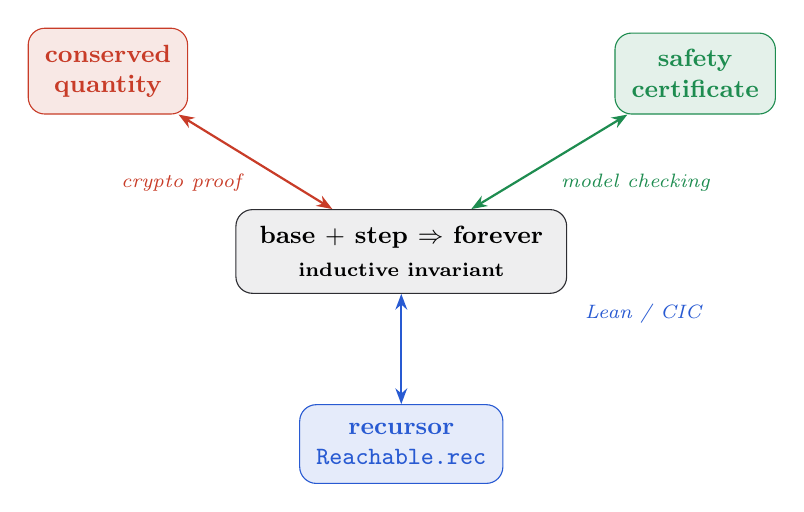
\begin{tikzpicture}[node distance=6mm]
  % central shape
  \node[chip,fill=ink!8,draw=ink,minimum width=42mm] (core)
    {base $+$ step $\Rightarrow$ forever\\[1pt]\scriptsize inductive invariant};
  % three costumes around it
  \node[chip,fill=crypto!12,draw=crypto,above left=12mm and 6mm of core,text=crypto]
    (c1) {conserved\\quantity};
  \node[chip,fill=mc!12,draw=mc,above right=12mm and 6mm of core,text=mc]
    (c2) {safety\\certificate};
  \node[chip,fill=cic!12,draw=cic,below=14mm of core,text=cic]
    (c3) {recursor\\\ttfamily Reachable.rec};
  \draw[eq,crypto] (core) -- (c1);
  \draw[eq,mc] (core) -- (c2);
  \draw[eq,cic] (core) -- (c3);
  \node[lbl,text=crypto,above left=1mm and -2mm of core]  {crypto proof};
  \node[lbl,text=mc,above right=1mm and -2mm of core] {model checking};
  \node[lbl,text=cic,below right=0mm and 1mm of core] {Lean / CIC};
\end{tikzpicture}
\caption{The pearl in one picture. The same invariant wears three costumes.
Each double arrow reads \emph{``same shape, different words''}. This paper draws
each costume and lets Lean check that they are the one shape.}
\label{fig:overview}
\end{figure}

% =========================================================================
\section{The pattern, stated once}

A \emph{transition system} is a set of start states and a step relation.
\emph{Reachable} is what you can get to. An \emph{inductive invariant} $P$ holds
at every start state and survives every step. The one load-bearing fact: such a
$P$ then holds at \emph{every} reachable state. That is the whole method ---
$P$ is the \emph{certificate}, the theorem is the \emph{check}.

\begin{figure}[H]
\centering
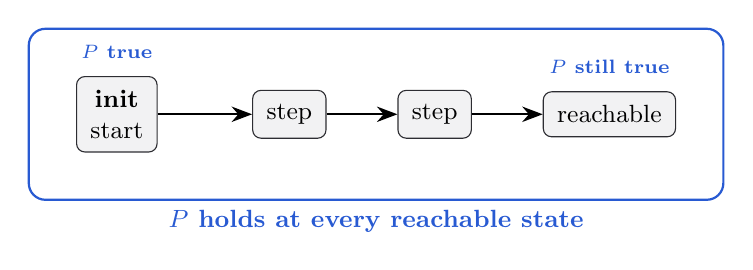
\begin{tikzpicture}[node distance=8mm]
  \node[box,fill=ink!6] (init) {\textbf{init}\\start};
  \node[box,fill=ink!6,right=12mm of init] (s1) {step};
  \node[box,fill=ink!6,right=9mm of s1] (s2) {step};
  \node[box,fill=ink!6,right=9mm of s2] (s3) {reachable};
  \draw[arr] (init) -- (s1);
  \draw[arr] (s1) -- (s2);
  \draw[arr] (s2) -- (s3);
  \begin{scope}[on background layer]
    \node[fit=(init)(s3),draw=cic,thick,rounded corners=6pt,inner sep=6mm,
      label={[cic,font=\small\bfseries]below:$P$ holds at every reachable state}]
      {};
  \end{scope}
  \node[cic,font=\scriptsize\bfseries,above=1mm of init] {$P$ true};
  \node[cic,font=\scriptsize\bfseries,above=1mm of s3] {$P$ still true};
\end{tikzpicture}
\caption{$P$ true at the start $+$ every step keeps $P$ $\;\Rightarrow\;$
$P$ true everywhere. The blue box is the theorem below.}
\label{fig:soundness}
\end{figure}

\begin{lstlisting}[style=lean]
structure InductiveInvariant (T : TransitionSystem State) (P : State -> Prop) : Prop where
  init_holds     : forall s, T.init s -> P s
  step_preserves : forall s s', P s -> T.step s s' -> P s'

theorem InductiveInvariant.reachable (h : InductiveInvariant T P) :
    forall s, Reachable T s -> P s
\end{lstlisting}

\noindent
Everything below is one instance of \lstinline[style=lean]|InductiveInvariant.reachable|.

% =========================================================================
\section{Costume 1 --- a conserved quantity in a crypto proof}

The pattern was \emph{spotted}, not invented, inside the proof of Dobbertin's
Theorem~6 over $\mathbb{F}_{2^n}$. Two polynomial sequences $A,B$ obey the same
two-step recurrence $s_{i+2}=u_i\,s_{i+1}+v_i\,s_i$. Their bilinear
\emph{cross term} is conserved (eq.~(11)):
\[
  A_i B_{i+1} + A_{i+1} B_i \;=\; z_i, \qquad z_{i+1}=v_i\, z_i .
\]

\begin{figure}[H]
\centering
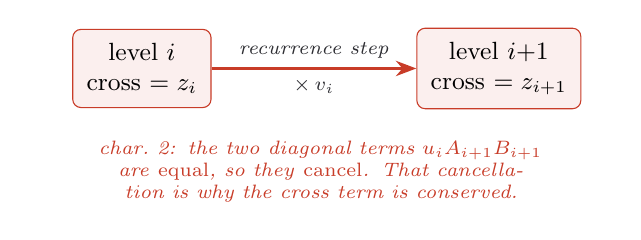
\begin{tikzpicture}[node distance=7mm]
  \node[box,fill=crypto!8,draw=crypto] (l0) {level $i$\\cross $=z_i$};
  \node[box,fill=crypto!8,draw=crypto,right=26mm of l0] (l1)
    {level $i{+}1$\\cross $=z_{i+1}$};
  \draw[arr,crypto] (l0) -- node[lbl,above]{recurrence step} node[lbl,below]{$\times\,v_i$} (l1);
  \node[lbl,text=crypto,below=8mm of $(l0)!0.5!(l1)$,text width=72mm]
    {char.~2: the two diagonal terms $u_i A_{i+1}B_{i+1}$ are \emph{equal}, so
     they \emph{cancel}. That cancellation is why the cross term is conserved.};
\end{tikzpicture}
\caption{Costume 1. The cross term is the invariant; one recurrence step
multiplies it by $v_i$. ``Holds at $i=0$, preserved by each step, therefore
holds for all $i$'' is exactly base $+$ step $\Rightarrow$ forever.}
\label{fig:crypto}
\end{figure}

\begin{lstlisting}[style=lean]
theorem cross_invariant (h : TwoStep u v A B) (i : N) :
    A (i+1) * B (i+2) + A (i+2) * B (i+1) = v i * (A i * B (i+1) + A (i+1) * B i)

theorem key_identity (h : TwoStep u v A B) (hz : forall i, z (i+1) = v i * z i)
    (h0 : A 0 * B 1 + A 1 * B 0 = z 0) (i : N) :
    A i * B (i+1) + A (i+1) * B i = z i          -- eq. (11), by induction on i
\end{lstlisting}

\noindent
\lstinline[style=lean]|key_identity| is a hand-rolled induction: base
(\lstinline[style=lean]|h0|), step (\lstinline[style=lean]|cross_invariant|),
done. The pattern is there --- but disguised as algebra.

% =========================================================================
\section{Costume 2 --- a safety certificate in model checking}

Give the shape its own vocabulary and it becomes the textbook safety recipe.
Two processes share one lock; safety is: never both in the critical section.

\begin{figure}[H]
\centering
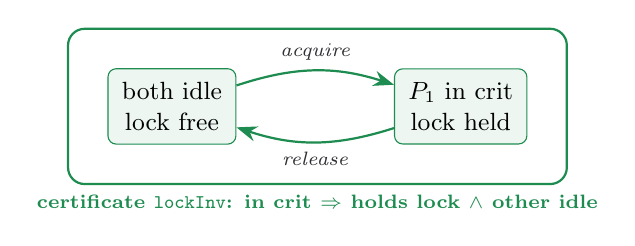
\begin{tikzpicture}[node distance=10mm]
  \node[box,fill=mc!8,draw=mc] (a) {both idle\\lock free};
  \node[box,fill=mc!8,draw=mc,right=20mm of a] (b) {$P_1$ in crit\\lock held};
  \draw[arr,mc] (a) to[bend left=18] node[lbl,above]{acquire} (b);
  \draw[arr,mc] (b) to[bend left=18] node[lbl,below]{release} (a);
  \begin{scope}[on background layer]
    \node[fit=(a)(b),draw=mc,thick,rounded corners=6pt,inner sep=5mm,
      label={[mc,font=\scriptsize\bfseries]below:%
      certificate \texttt{lockInv}: in crit $\Rightarrow$ holds lock $\wedge$ other idle}]{};
  \end{scope}
\end{tikzpicture}
\caption{Costume 2. The invariant \texttt{lockInv} is the certificate; feeding it
to \texttt{safety\_via\_invariant} discharges mutual exclusion. Same shape as
Fig.~\ref{fig:crypto}, familiar example.}
\label{fig:mutex}
\end{figure}

\begin{lstlisting}[style=lean]
theorem mutualExclusion_reachable (s : St) (hs : Reachable mutexSystem s) :
    mutualExclusion s :=
  safety_via_invariant lockInv_inductive lockInv_imp_mutualExclusion s hs
\end{lstlisting}

% =========================================================================
\section{Costume 3 --- the recursor of an inductive type}

Why is \lstinline[style=lean]|InductiveInvariant.reachable| \emph{true}? Because
\lstinline[style=lean]|Reachable| is an ordinary Lean inductive: its two
constructors are exactly the two rules ``start'' and ``step''. Soundness is
nothing more than its auto-generated recursor, fed the invariant's two fields.

\begin{lstlisting}[style=lean]
inductive Reachable (S : System sigma) : sigma -> Prop
  | start : S.init s -> Reachable S s                        -- rule 1  (= init_holds)
  | step  : Reachable S s -> S.step s s' -> Reachable S s'   -- rule 2  (= step_pres)
\end{lstlisting}

\begin{figure}[H]
\centering
\begin{tikzcd}[column sep=large, row sep=small]
  \textcolor{cic}{\texttt{init\_holds}} \arrow[dr] & \\
  & \boxed{\texttt{Reachable.rec}} \arrow[r] & \textcolor{mc}{P \text{ at every reachable state}} \\
  \textcolor{cic}{\texttt{step\_pres}} \arrow[ur] &
\end{tikzcd}
\caption{Costume 3, as a commuting picture. The two invariant fields are the two
arguments the recursor \lstinline[style=lean]|Reachable.rec| takes; its output is
soundness. Nothing else is needed.}
\label{fig:recursor}
\end{figure}

\begin{lstlisting}[style=lean]
-- soundness, written by hand-applying the recursor:
theorem Inductive.reachable' (h : Inductive S P) : forall s, Reachable S s -> P s :=
  fun _ hs => Reachable.rec (fun hi => h.init_holds _ hi)
                            (fun _ hstep ih => h.step_pres _ _ ih hstep) hs

-- the "by induction" proof and the raw-recursor proof are the SAME term:
example (h : Inductive S P) : Inductive.reachable h = Inductive.reachable' h := rfl
\end{lstlisting}

\begin{artifact}
\small\centering
The \lstinline[style=lean]|rfl| is the pearl's punchline: \texttt{by induction}
elaborates to \texttt{Reachable.rec}. Model-checking soundness is not merely
\emph{proved by} induction --- it \emph{is} CIC induction.
\lstinline[style=lean]|InductiveInvariant.reachable| depends on \textbf{no axioms}.
\end{artifact}

% =========================================================================
\section{Closing the loop --- the crypto identity, re-derived}

The circle closes when we re-tell Costume~1 in the vocabulary of Costume~2. Make
the state a sliding window $(i,A_i,A_{i+1},B_i,B_{i+1})$ and the step the
recurrence. Then the cross term is an inductive invariant, and eq.~(11) drops out
of the \emph{generic} soundness theorem --- a faithful ``morphism'' from the
crypto proof to the model-checking core.

\begin{figure}[H]
\centering
\begin{tikzcd}[column sep=6.5em, row sep=large]
  \textcolor{crypto}{\substack{\text{hand-rolled}\\\texttt{key\_identity}}}
    \arrow[r, "\text{recognise}"] \arrow[dr, "\text{induction}"']
  & \textcolor{cic}{\substack{\text{generic}\\\texttt{InductiveInvariant.reachable}}}
    \arrow[d, "\text{instantiate}"] \\
  & \textcolor{mc}{\substack{\text{eq.~(11) for all }i\\\texttt{key\_identity\_via\_reachable}}}
\end{tikzcd}
\caption{The loop commutes. The identity spotted by hand (top-left) and the same
identity produced by the generic machinery (bottom) agree; recognising the
pattern is the diagonal that makes them one.}
\label{fig:loop}
\end{figure}

\begin{lstlisting}[style=lean]
theorem cross_is_inductiveInvariant (hz : forall i, z (i+1) = v i * z i) :
    InductiveInvariant (recSystem u v z) (crossInv z)     -- cross term is an invariant

theorem key_identity_via_reachable ... (i : N) :
    A i * B (i+1) + A (i+1) * B i = z i                        -- eq. (11), now an instance
  := cross_holds_of_reachable ... (windowState_reachable ... i)
\end{lstlisting}

% =========================================================================
\section{Three costumes, one table}

\begin{table}[H]
\centering
\caption{The one shape, read three ways. Every row is a machine-checked theorem.}
\label{tab:costumes}
\renewcommand{\arraystretch}{1.25}
\small
\begin{tabular}{@{}llll@{}}
\toprule
 & \textcolor{crypto}{\textbf{crypto}} & \textcolor{mc}{\textbf{model checking}} & \textcolor{cic}{\textbf{Lean / CIC}}\\
\midrule
state      & level $i$, window $A,B$ & lock $+$ two locations & a term of \texttt{Reachable}\\
invariant  & cross term $=z_i$       & \texttt{lockInv}       & the motive $P$\\
base       & eq.~(11) at $i=0$       & both idle, lock free   & \texttt{init\_holds}\\
step       & char.~2 cancellation    & acquire / release      & \texttt{step\_pres}\\
conclusion & eq.~(11) for all $i$    & never both in crit     & $P$ everywhere reachable\\
theorem    & \texttt{key\_identity}  & \texttt{mutualExclusion\_} & \texttt{InductiveInvariant.}\\
           & \texttt{\_via\_reachable}& \texttt{reachable}     & \texttt{reachable} $=$ \texttt{.rec}\\
\bottomrule
\end{tabular}
\end{table}

% =========================================================================
\section{What transfers, and what this is not}

\paragraph{What transfers.} Whenever you can name a quantity that (i) holds at the
start and (ii) is preserved by one step, you already have a proof for the whole
run --- and, in a proof assistant, that proof is free: it is the recursor. The
skill is \emph{recognition}, not machinery.

\paragraph{Honest scope.} This is the soundness \emph{kernel} certifying model
checking rests on --- done by hand in a proof assistant. It is not an automated
or SMT-backed checker and does not explore millions of states. Real tools scale
this to large systems; here it is deliberately small, so the core is fully
understood and fully checked.

\begin{artifact}
\textbf{Artifact.} Lean~4 / Mathlib (\texttt{v4.28.0}). Builds with
\texttt{lake build}, no \lstinline[style=lean]|sorry|.
Anchors: \lstinline[style=lean]|InductiveInvariant.reachable| (no axioms);
\lstinline[style=lean]|Inductive.reachable = Inductive.reachable'| by
\lstinline[style=lean]|rfl|; \lstinline[style=lean]|key_identity_via_reachable|
re-derives eq.~(11). Six short files, one per section.
\end{artifact}

% =========================================================================
\begin{table}[H]
\centering
\caption{Mindful design log (Ellen Langer style): a usual ``default'' of pearl
writing, and the option taken here once it is noticed as \emph{just} a default.}
\label{tab:mindful}
\renewcommand{\arraystretch}{1.15}
\small
\begin{tabular}{@{}ll@{}}
\toprule
\textbf{usual default} & \textbf{option taken here}\\
\midrule
front-load prose motivation      & open with Fig.~\ref{fig:overview}; captions motivate\\
write proofs in text             & proofs as commuting diagrams (Figs.~\ref{fig:recursor},\ref{fig:loop})\\
a new result                     & re-derivation-as-pearl: recognise a known shape\\
figures illustrate the text      & text annotates the figures\\
related work is a section        & positioned in one table (Table~\ref{tab:costumes})\\
contributions as a bullet list   & one overview figure, three costumes\\
fill the page limit              & brevity is the contribution\\
\bottomrule
\end{tabular}
\end{table}

\paragraph{Acknowledgement.} The Lean development was carried out with
machine assistance; all statements are checked by the Lean kernel.

\end{document}
